\chapter{Metodologia przeprowadzonych badań}
\label{cha:metodologia}

W rozdziale tym zaprezentowano metodologię przeprowadzania badań metod detekcji obiektu pod względem zarówno jakościowym jak i czasowym.

\section{Implementacja}
\label{sec:implementacja}

Przedstawiona w niniejszym rozdziale metodologia wraz z metodami zaprezentowanymi w rozdziałach \ref{cha:deskryptory} i \ref{cha:laczenie} zaimplementowana została w języku C++, przy użyciu biblioteki OpenCV2 \cite{opencv_library}. Biblioteka ta, poza tym że udostępnia możliwość wykonywania wielu operacji na obrazach z poziomu jej interfejsu, udostępnia także wiele metod uczenia maszynowego, w tym Support Vector Machine, która została wykorzystana~w~tej pracy.

Implementacja została udostępniona na licencji GNU/GPL, na portalu GitHub, pod adresem \cite{GitHub_Sauce}.

\section{Wykorzystywany zestaw danych}
\label{sec:dane}
Do badania działania metod detekcji obiektów wybrano bazę danych opracowaną we francuskim instytucie INRIA, która powstała w trakcie badań nad pracą \cite{Dalal05}, opisującą wówczas nowe podejście do detekcji ludzi na obrazie.
Baza ta zawiera obrazy przeznaczone do uczenia i testowania metod detekcji ludzi na obrazie podzielone na zbiory próbek: \textbf{pozytywnych}, gromadzących ponad 1500 obrazów zawierających sylwetkę człowieka wraz z ich lustrzanymi odbiciami oraz \textbf{negatywnych}, składających się z blisko 1700 obrazów niezawierających takiej sylwetki.

Baza ta powstała w wyniku wykorzystania już istniejących zbiorów obrazów, przypadkowych obrazów znalezionych w sieci Internet, a także z prywatnych zbiorów autorów, ze zdjęć wykonywanych w długim okresie czasu.
W przypadku sylwetek ludzkich, wiele z nich zostało wyodrębnionych ze zdjęć, na których znalazły się one nieświadomie (byli to np. przechodnie w tle) i w związku z tym można mówić~o~braku przyjętej przez nich specyficznej pozy.
Obrazy obecne w zbiorze pozytywnym, zostały znormalizowane i ujednolicone w taki sposób, że zawierają one ludzką sylwetkę w centrum obrazu o rozmiarze 64x128 pikseli (część zbioru zawiera dodatkowy margines 16 lub 3 pikseli dla każdej z krawędzi obrazu, w~celu uniknięcia warunków brzegowych). Przykładowe obrazy z pozytywnego zbioru zaprezentowano na rysunku \ref{fig:inria}.

\begin{figure}[htb]
\centering
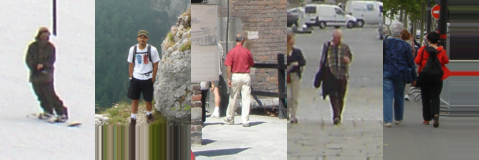
\includegraphics[width=0.8\textwidth]{ch3_inria.png}
\caption{Przykłady pozytywnych próbek ze zbioru INRIA}
\label{fig:inria}
\end{figure}

Ponadto, wszystkie obrazy będące częścią pozytywnego zbioru próbek, zawierają dodatkowy opis lokalizacji osób na nim w formacie \textit{Pascal Challenge} \cite{Pascal_Challenge}. Pozwala to na sprawdzenie poprawności działania finalnej metody.
Autorzy zbioru nie zapewnili negatywnego zbioru danych, odpowiadającego pozytywnym próbkom o rozmiarze 64x128 pikseli, pozostawiając wybór okien tego rozmiaru z większych negatywnych obrazów autorom konkretnej implementacji. Propozycja wyboru takich negatywnych okien została zaprezentowana w rozdziale \ref{sec:podzial}.


\section{Klasyfikator - Support Vector Machine}
\label{sec:svm}

Zadanie budowy klasyfikatora polega na podziale zbioru danych na dwa zestawy: treningowy i testowy. Każda próbka w zbiorze treningowym dostaje etykietę – jest próbką pozytywną, reprezentującą zajście jakiegoś zjawiska, lub negatywną – wtedy reprezentuje brak jego zajścia. Dla każdej próbki z obu zestawów wyliczana jest wartość deskryptora cech, po czym wraz z odpowiednią etykietą, pozytywną lub negatywną, przekazywana jest ona do klasyfikatora w celu wytrenowania go. Po tym kroku, możliwe jest dokonywanie klasyfikacji, na bardzo podobnej zasadzie do fazy treningowej. Klasyfikator na podstawie przekazanego wektora cech przewiduje do której z dwóch klas obiektów należy próbka – pozytywnej czy negatywnej.

Support Vector Machine (SVM) jest bardzo często używaną i dającą dobre wyniki techniką, statystycznego uczenia maszynowego. Metoda zaproponowana przez dwójkę C. Cortesa i V. Vapnika w pracy \cite{Cortes95}, z matematycznego punktu widzenia jest problemem optymalizacyjnym postaci:\\

\begin{enumerate}[label=\arabic*)]
  \item \rule{0pt}{1pt}\vspace*{-12pt}
    \begin{equation*} 
     \min_{\bm{w},b,\xi} \frac{1}{2} \bm{w}^T\bm{w} + C\sum_{i=1}^{l} \xi_{i}
    \end{equation*}
    przy ograniczeniach:
  \item \rule{0pt}{1pt}\vspace*{-12pt}
  	\begin{equation*} 
     {l}y_{i}(\bm{w}^{T}\phi(\bm{x}_i)+b)\geq 1-\xi_{i}
    \end{equation*}
   \item \rule{0pt}{1pt}\vspace*{-12pt}
  	\begin{equation*} 
     \xi_{i} \geq 0
   	\end{equation*}
   	gdzie zbiór treningowy to zbiór par
  \item \rule{0pt}{1pt}\vspace*{-12pt}
  	\begin{equation*} 
     (\bm{x}_i, y_i), i \in \{1, ..., l\}
   	\end{equation*}
   	wektorem cech dla danej próbki jest
   	\item \rule{0pt}{1pt}\vspace*{-12pt}
  	\begin{equation*} 
     \bm{x}_i \in R^n
   	\end{equation*}
   	a identyfikatorem klasy i-tej próbki jest
   	\item \rule{0pt}{1pt}\vspace*{-12pt}
  	\begin{equation*} 
     y_i \in \{-1, 1\}
   	\end{equation*}
\end{enumerate}

Intuicyjna ilustracja metody, na przykładzie dwuwymiarowego wektora cech została zaprezentowana na rysunku \ref{fig:svm}.

Wektory cech odwzorowywane są na przestrzeń o większej liczbie wymiarów poprzez funkcję $\phi$. Zadaniem SVM jest znalezienie takiego podziału hiperpłaszczyzny, jak najbardziej odległej od granic umiejscowienia wektorów obu klas. Funkcja $K(\bm{x}_i, \bm{x}_j) = \xi(\bm{x}_i)^T\xi(\bm{x}_j)$ nazywana jest funkcją jądra SVM (\textit{kernel}).

Najczęściej używanymi funkcjami są:
\begin{enumerate}[label=\arabic*)]
  \item \rule{0pt}{1pt}\vspace*{-12pt}
  funkcja liniowa:
    \begin{equation*} 
     K(\bm{x}_i, \bm{x}_j) = \bm{x}_i^T\bm{x}_j
    \end{equation*}
  \item \rule{0pt}{1pt}\vspace*{-12pt}
  funkcja wielomianowa:
    \begin{equation*} 
     K(\bm{x}_i, \bm{x}_j) = (\gamma\bm{x}_i^T\bm{x}_j+r)^d,  \gamma > 0
    \end{equation*}
  \item \rule{0pt}{1pt}\vspace*{-12pt}
  funkcja RBF:
    \begin{equation*} 
    K(\bm{x}_i, \bm{x}_j) = e^{-\gamma\Vert\bm{x}_i-\bm{x}_j\Vert^2},  \gamma > 0
    \end{equation*}
  \item \rule{0pt}{1pt}\vspace*{-12pt}
  esica (\textit{sigmoid}):
    \begin{equation*} 
    K(\bm{x}_i, \bm{x}_j) = tanh(-\gamma\bm{x}_i^T\bm{x}_j+r)
    \end{equation*}
  	gdzie $\gamma, r, d$ są parametrami.
\end{enumerate}

\begin{figure}[htb]
\centering
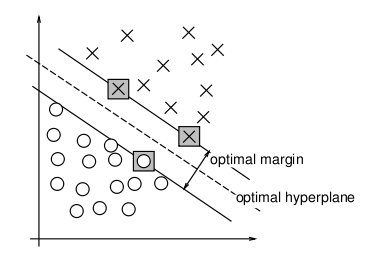
\includegraphics[width=0.5\textwidth]{ch3_svm.png}
\caption{Przykład budowy klasyfikatora dla wektora dwóch cech. \textit{Źródło: \cite{Cortes95}}}
\label{fig:svm}
\end{figure}

Zjawiskiem niepożądanym przy treningu klasyfikatora jest jego przetrenowanie. Do takiej sytuacji dochodzi w momencie, gdy w zbiorze treningowym którejś z klas znajduje się zbyt duża liczba wektorów leżących bardzo blisko realnej granicy. Wtedy hiperpłaszczyzna wyznaczona przez SVM jest dobrze dopasowana do tych skrajnych w przypadku jeden klasy i próbek drugiej klasy, leżących dalej od realnej granicy. W konsekwencji, wyznaczona granica może leżeć dość daleko od realnej.

\section{Podział zbioru danych}
\label{sec:podzial}

Jak wspomniano w \ref{sec:dane}, autorzy bazy danych INRIA zapewnili odpowiednio wykadrowany pozytywny zbiór treningowy i testowy, zawierający próbki o rozmiarze zgodnym z oknem detekcji, zawierające postać ludzką w samym jej centrum. Zbiory te zostały podzielone w stosunku 2416 próbek treningowych i 626 próbek testowych.
W przypadku zbiorów negatywnych, które zostały podzielone w stosunku 1218 próbek treningowych i 453 próbki testowe, mamy do czynienia z pełnymi zdjęciami w różnych rozdzielczościach. W tym przypadku, autorzy zbioru pozostawili dowolność w konstrukcji wykadrowanych zbiorów autorom konkretnej implementacji.

Proponowane podejście do generacji zarówno zbioru treningowego i testowego jest następujące.
Z~każdego obrazu ze zbioru negatywnego generowane są cztery okna o rozmiarze 64x128 pikseli - trzy całkowicie losowe i jedno wybierane według następującej zasady:
na całym obrazie stosowany jest operator Sobela w kierunkach poziomym i pionowym, wybierane jest to okno, dla którego suma wartości bezwzględnych takiej operacji jest maksymalna. Innymi słowy, wybierane jest okno, które na całym obrazie dominuje pod względem ilości krawędzi.

\begin{figure}[htb]
\centering
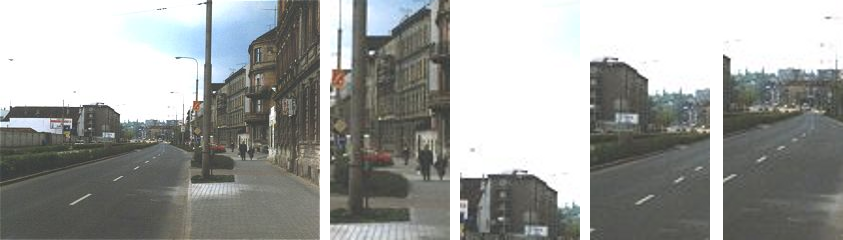
\includegraphics[width=0.8\textwidth]{ch3_sobel.png}
\caption{Negatywny obraz ze zbioru danych i wygenerowane na jego podstawie negatywne dane treningowe, od lewej: na podstawie wyniku filtru Sobela i 3 losowe okna}
\label{fig:sobel}
\end{figure}

Takie podejście powinno pozwolić na generację wiarygodnego klasyfikatora. Użyte negatywne dane, zarówno te wybrane do treningu klasyfikatora jak i jego walidacji, będą zróżnicowane pod względem ilości krawędzi, czyli cechy głównie wykorzystywanej przez prezentowane deskryptory do opisu obiektów.

Przykład negatywnego obrazu ze zbioru wraz z wygenerowanymi na jego podstawie oknami został przedstawiony na rys. \ref{fig:sobel}.

\section{Trening i walidacja}
\label{sec:trening}

Wytrenowanie klasyfikatora Support Vector Machine polega na konstrukcji wektora próbek - w kontekście tej pracy jest to wynik obliczenia danego deskryptora cech lub wynik połączenia kilku deskryptorów. Jeżeli wyjściem z deskryptora jest macierz, dokonuje się ''rozwinięcia'' tej macierzy w wektor poprzez połączenie ze sobą kolejnych wierszy lub kolumn. Przyjęty sposób zmiany rozmiaru macierzy nie ma znaczenia, gdyż każdy element wektora reprezentuje niezależną od innych cechę, ważne jest natomiast by zachować konsekwencję zarówno w trakcie budowy takiego wektora w fazie treningu jak i w fazie klasyfikacji. Każdemu wektorowi próbki przypisana jest etykieta oznaczająca klasę, do jakiej on należy. W pracy przyjęto następujący sposób etykietowania: do klasy \textit{0} należą wszystkie wektory, które są efektem zastosowania deskryptora na próbce nie zawierającej sylwetki ludzkiej, z kolei do klasy \textit{1} na próbce z sylwetką ludzką.

W pracy do budowy klasyfikatora użyto implementacji Support Vector Machine udostępnionej w~bibliotece OpenCV2. W trakcie badań uwzględniono budowę klasyfikatora z użyciem liniowego odwzorowania (tzw. \textit{kernel}) wektora próbki.

Klasyfikator nie posiada, w przeciwieństwie do danych ze zbioru treningowego, żadnych informacji na temat klasy, do jakiej należą poddawane przez nas klasyfikacji próbki ze zbioru testowego, dlatego też pierwszym sprawdzeniem poprawności działania klasyfikatora powinno być zastosowanie go na przygotowanym wcześniej zbiorze testowym. Znajomość procentowej poprawności odpowiedzi klasyfikatora pozwala krytycznie spojrzeć na poprawność zastosowanej metody i zauważyć pewne problemy jak np. przetrenowanie klasyfikatora, zanim dokona się sprawdzenia działania metody na rzeczywistych, bardziej złożonych danych.

W przypadku detekcji obiektów, takich jak ludzie, na obrazie, za zadowalający można przyjąć klasyfikator zapewniający ok. 90\% poprawności klasyfikacji zarówno na pozytywnym jak i negatywnym zbiorze testowym.

W przypadku Support Vector Machine, walidacja jest szczególnie ważna w przypadkach, w których używa się funkcji odwzorowującej wektor na wyższy wymiar. Wynika to z faktu, że dobór parametrów funkcji mapującej dokonywany jest na podstawie wyniku skuteczności klasyfikatora na zbiorze testowym.

\section{Dotrenowanie klasyfikatora}
\label{sec:dotrenowanie}

Skorzystanie z samego, wcześniej przygotowanego zbioru treningowego, może nie dawać zadowalających rezultatów w przypadku dokonywania klasyfikacji na rzeczywistych obrazach. Najczęstszą tego przyczyną jest fałszywa pozytywna detekcja w oknach, w których obserwowalne są kształty w pewnym sensie zbliżone do ludzkich, np. zawierające długie pionowe równoległe linie.
Przykłady kilku takich detekcji przedstawiono na rysunku \ref{fig:fp}.

W celu poprawienia skuteczności działania klasyfikatora dokonuje się jego dotrenowania. Polega ono na wykryciu fałszywych pozytywnych wskazań na testowym zbiorze obrazów rzeczywistych, a~następnie ponownym wytrenowaniu klasyfikatora, tym razem jednak ze zbiorem negatywnych próbek powiększonym o właśnie te niepoprawne detekcje.

\begin{figure}[htb]
\centering
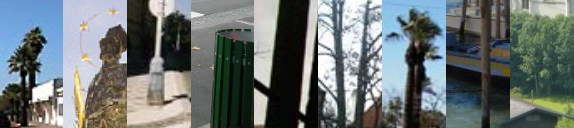
\includegraphics[width=0.8\textwidth]{ch3_fp.png}
\caption{Przykłady fałszywie pozytywnych detekcji}
\label{fig:fp}
\end{figure}

Negatywny zbiór treningowy jest jednak powiększany nie przez całość, a tylko część fałszywych pozytywnych okien wygenerowanych w fazie testu. Badania pokazały, że zbyt duży udział takich próbek w~całym negatywnym zbiorze treningowym prowadzi do zjawiska przetrenowania klasyfikatora, opisanego w \ref{sec:svm}. W związku z tym pierwotny zbiór treningowy powiększany jest np. o 1/3 losowych, wygenerowanych detekcji tego typu, po czym następuje ponowny trening klasyfikatora.


\section{Detekcja w przesuwnym oknie}
\label{sec:okno}

Ze względu na fakt, że rzeczywiste obrazy, na których dokonuje się detekcji obiektów, mogą mieć różne rozdzielczości, krokiem wymaganym na samym początku procesu detekcji, po wczytaniu obrazu powinna być pewna jego normalizacja. W niniejszej pracy, wszystkie obrazy wejściowe zmniejszane są do wysokości 600 pikseli, z zachowaniem proporcji. Dopiero na takim obrazie rozpoczynana jest detekcja obiektów.

Biorąc pod uwagę wymagania klasyfikatora, polegające na tym że klasyfikacji można poddać tylko i~wyłącznie okno o takim samym rozmiarze jak próbki poddane treningowi, niemożliwa jest klasyfikacja całego obrazu wejściowego w jednym kroku. Aby dokonać detekcji stosuje się koncepcję tzw. przesuwnego okna. Polega ona na podziale obrazu wejściowego na fragmenty o rozmiarze zgodnym z wielkością okna klasyfikowanego. Dla każdego takiego fragmentu dokonuje się osobnej, niezależnej od innych fragmentów, klasyfikacji. Takie niezłożone podejście ma jednak swoją wadę - ze względu na dużą liczbę testowanych okien w obrębie jednego obrazu, nawet wysoka celność klasyfikatora w przypadku próbek negatywnych może prowadzić do dużej liczby fałszywie pozytywnych detekcji (FP - \textit{False Positives}). Jest to zjawisko polegające na zaklasyfikowaniu próbki jako prawdziwej, podczas gdy w rzeczywistości jest ona fałszywa.

W badaniach przeprowadzonych w niniejszej pracy dokonano detekcji w oknie o rozmiarze 64x128 pikseli. Okno było przesuwane co 32 piksele w poziomie i co 64 piksele w pionie.

\section{Skalowanie obrazu testowanego}
\label{sec:skalowanie}

Biorąc pod uwagę to, że rzeczywiste obrazy testowane są zwykłymi fotografiami, zrobionymi w różnych okolicznościach, sylwetki ludzkie na nich obecne nie podlegają żadnej normalizacji.
Oznacza to, że człowiek, który powinien zostać wykryty na obrazie, może zajmować różną jego część, w zależności od tego jak daleko od miejsca zrobienia zdjęcia znajdował się w danej chwili. W testowym zbiorze danych obecne są przykłady zdjęć, w których postać znajduje się na pierwszym planie i jest obecna na prawie całej wysokości obrazu. Znajduje się w nim również wiele obrazów, w których postaci znajdują się w tle i wypełniają stosunkowo małą powierzchnię obrazu.

Przy stałej wielkości okna detekcji, która określona jest przez sposób budowy deskryptora cech w~trakcie treningu klasyfikatora, w celu wykrycia obiektów o różnej wielkości na obrazie, konieczne jest zatem kilkukrotne przeskalowanie obrazu testowanego.

\begin{figure}[htb]
\centering
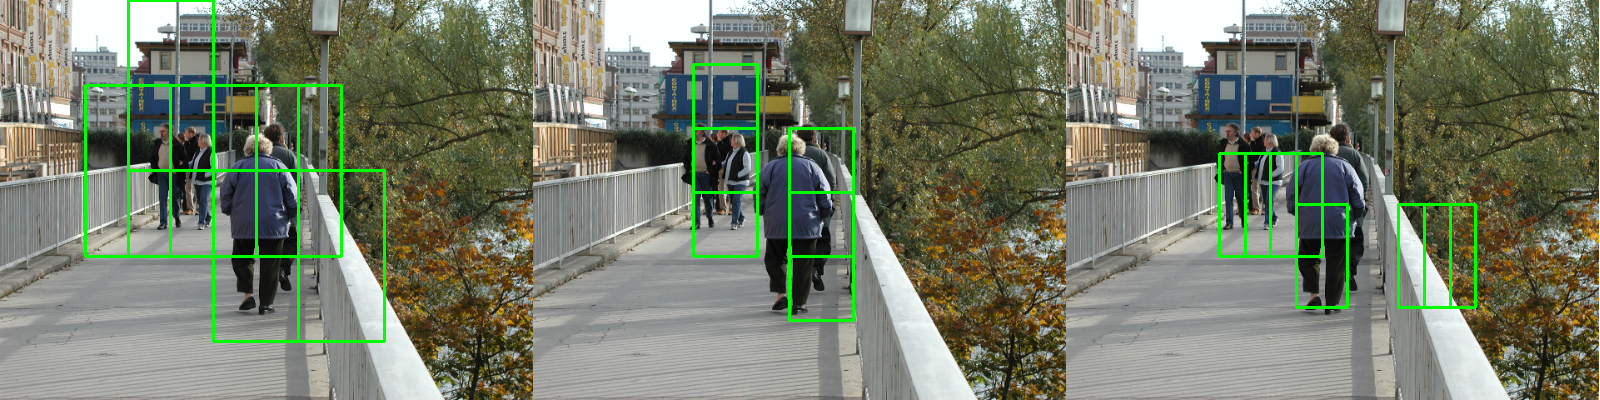
\includegraphics[width=0.8\textwidth]{ch3_scales.png}
\caption{Przykłady detekcji na obrazie testowanych w~skalach kolejno: \textbf{0.75}, \textbf{1} i \textbf{1.25}}
\label{fig:skale}
\end{figure}

Testy wykonane na obrazach przeskalowanych w skalach 0.25, 0.5, 0.75, 1 i 1.25 wykazały, że ostatecznie wystarczające będzie przeskalowanie obrazów testowanych w skalach \textbf{0.5}, \textbf{0.75} i \textbf{1}. W przypadku skali 0.25, pożądany obiekt był wykrywany w bardzo niewielkiej ilości przypadków, z kolei dla skali 1.25, ekstrakcja okien detekcji z dużym zbliżeniem, powodowała klasyfikację próbek z wieloma szczegółami obecnymi w otoczeniu. Konsekwencją tego była generacja znacznej liczby FP.

Na rysunku \ref{fig:skale} znajdują się przykłady detekcji obiektów na przeskalowanych obrazach testowych w skalach 0.75, 1 i 1.25.

\section{Eliminacja redundantnych detekcji}
\label{sec:eliminacja}

Detekcja obiektu na kilku przeskalowanych obrazach, a także mały krok przesunięcia przesuwnego okna może prowadzić do sytuacji, w której ten sam obiekt zostanie wykryty kilkukrotnie.
Aby w ostatecznym wyniku detekcji uniknąć tego typu sytuacji przyjęto następujący algorytm postępowania:
\\

\begin{algorithm}[H]
 \SetAlgoLined
 \KwData{zbiór okien detekcji zaklasyfikowanych pozytywnie przez klasyfikator w postaci \{współrzędne okna, pewność detekcji\}}
 \KwResult{zbiór ostatecznych okien detekcji}
 strefa zabroniona := $\oslash$\;
 finalny zbiór okien detekcji := $\oslash$\;
 posortuj wejściowe okna detekcji malejąco względem pewności detekcji\;
 
 \ForEach{okno}{
 	\If{okno = \{współrzędne, pewność\} $\notin$ strefa zabroniona}{
 	finalny zbiór okien detekcji := finalny zbiór okien detekcji $\cup$ okno\;
 	strefa zabroniona := strefa zabroniona $\cup$ współrzędne\;
 	}
 }
 \Return{finalny zbiór okien detekcji}
 \\
 \caption{Algorytm usuwania redundantnych detekcji}
\end{algorithm}

\begin{figure}[htb]
\centering
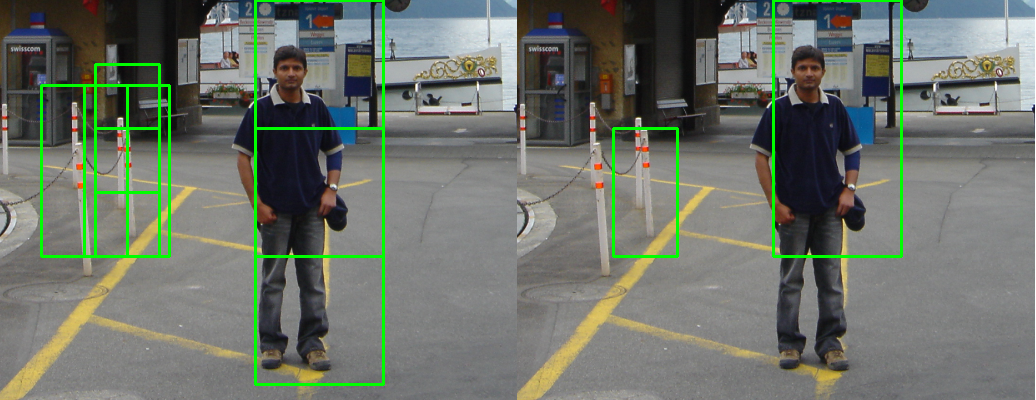
\includegraphics[width=0.8\textwidth]{ch3_redundant.png}
\caption{Po lewej obraz z redundantnymi detekcjami, po prawej po usunięciu redundantnych detekcji}
\label{fig:redundancje}
\end{figure}

Przykład pierwotnych, redundantnych okien detekcji wraz z oknami po redukcji, znajduje się na rysunku \ref{fig:redundancje}.

\section{Walidacja z wykorzystaniem danych rzeczywistych}
\label{sec:rzeczywiste}

Dzięki udostępnieniu, wraz z pozytywnymi zestawami (zawierającymi
przynajmniej jedną sylwetkę ludzką), zarówno zdjęć testowych jak i
treningowych w bazie INRIA plików opisu umiejscowienia tychże na
obrazie w formacie \textit{Pascal Challenge}, możliwe było zbudowanie
automatycznego narzędzia pozwalającego na przebadanie skuteczności
działania metody na obrazach jakie w rzeczywistości zostaną poddane
procesowi detekcji.

Przykładowy obraz z pozytywnego zbioru testowego z zaznaczonymi występującymi na nim sylwetkami ludzkimi znajduje się na rysunku \ref{fig:pascal}, z kolei odpowiadający mu plik
opisującym na nim obecność sylwetek ludzkich w formacie \textit{Pascal
Challenge} znajduje się poniżej (oryginalny obraz ma rozmiar 953 x 828
pikseli).

\begin{figure}[htb]
\centering
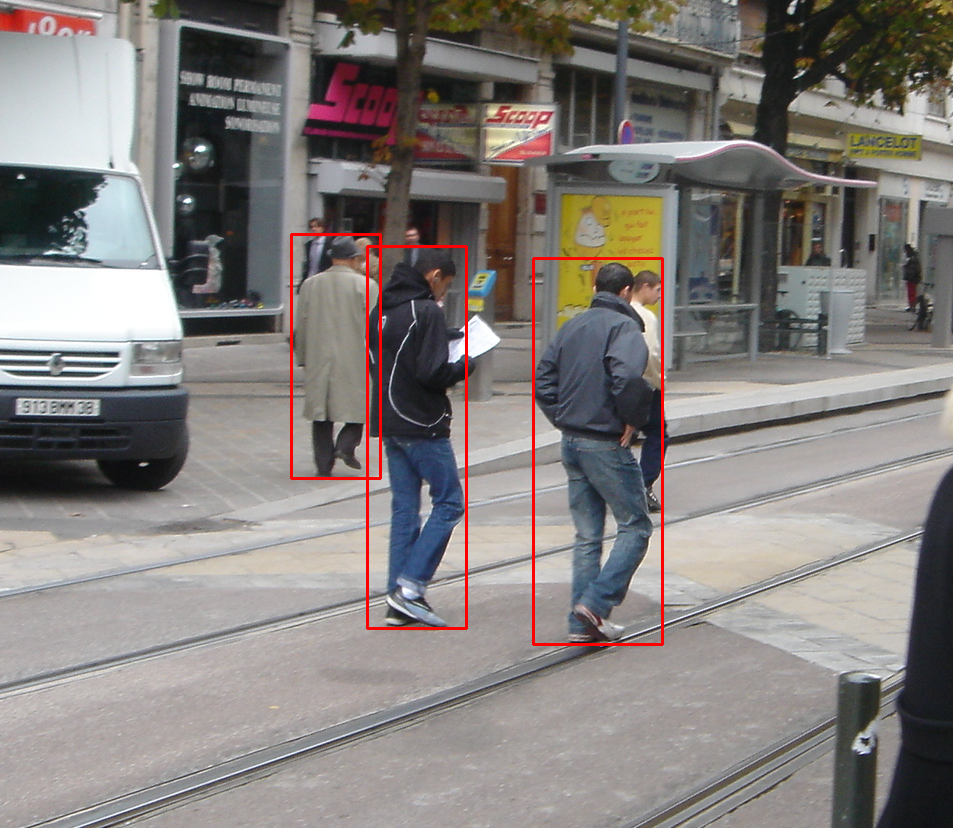
\includegraphics[width=0.8\textwidth]{ch4_pascal.png}
\caption{Przykładowy obraz z pozytywnego zbioru testowego z zaznaczonymi występującymi na nim postaciami na podstawie informacji zawartych w odpowiadającym mu pliku w formacie \textit{Pascal Challenge}}
\label{fig:pascal}
\end{figure}

\begin{lstlisting}
# PASCAL Annotation Version 1.00

Image filename : "Test/pos/crop001514.png"
Image size (X x Y x C) : 953 x 828 x 3
Database : "The INRIA Rhone-Alpes Annotated Person Database"
Objects with ground truth : 3 { "PASperson" "PASperson" "PASperson" }

# Note that there might be other objects in the image
# for which ground truth data has not been provided.

# Top left pixel co-ordinates : (0, 0)

# Details for object 1 ("PASperson")
# Center point -- not available in other PASCAL databases -- refers
# to person head center
Original label for object 1 "PASperson" : "UprightPerson"
Center point on object 1 "PASperson" (X, Y) : (436, 280)
Bounding box for object 1 "PASperson" (Xmin, Ymin) - (Xmax, Ymax) : (367, 246) - (467, 629)

# Details for object 2 ("PASperson")
# Center point -- not available in other PASCAL databases -- refers
# to person head center
Original label for object 2 "PASperson" : "UprightPerson"
Center point on object 2 "PASperson" (X, Y) : (345, 263)
Bounding box for object 2 "PASperson" (Xmin, Ymin) - (Xmax, Ymax) : (291, 234) - (381, 479)

# Details for object 3 ("PASperson")
# Center point -- not available in other PASCAL databases -- refers
# to person head center
Original label for object 3 "PASperson" : "UprightPerson"
Center point on object 3 "PASperson" (X, Y) : (609, 293)
Bounding box for object 3 "PASperson" (Xmin, Ymin) - (Xmax, Ymax) : (533, 258) - (663, 645)
\end{lstlisting}

Jak wspomniano w rozdziale \ref{sec:okno}, często w systemach
wizyjnych, których zadaniem jest wykrycie obiektów na obrazie, do detekcji stosowana jest koncepcja okna przesuwanego wzdłuż i wszerz testowanego obrazu. Klasyfikator klasyfikuje każde z nich
jako pozytywne lub negatywne. W celu stwierdzenia, czy rezultat, jaki uzyskano dla
okna w wyniku klasyfikacji jest poprawny w~kontekście
informacji zawartych w pliku zawierającym informacje o sylwetkach
obecnych na obrazie, przyjęto następującą procedurę postępowania:

\begin{algorithm}[H]
 \SetAlgoLined
 \KwData{współrzędne okna detekcji, współrzędne prostokątów opisujących obiekty obecne na obrazie}
 \KwResult{wartość logiczna odpowiadająca na pytanie, czy klasyfikacja jest poprawna czy też nie}
 \ForEach{prostokąt opisujący obiekt} {
 	\If{okno ma przynajmniej jeden punkt wspólny z prostokątem} {
 		\If{$pole(okno \cap prostokat) \geq \frac{1}{2} min(pole(okno), pole(prostokat))$} {
 			\Return{true}\;
 		}
 	}
 }
 \Return{false}
 \\
 \caption{Algorytm sprawdzenia czy okno poddane detekcji jest w rzeczywistości pozytywne czy negatywne}
\end{algorithm}

Na rysunku \ref{fig:detections} zaprezentowano przykład działania powyższego algorytmu, dokonując detekcji wykonywanych na kilkukrotnie przeskalowanym obrazie, bez uwzględnienia algorytmu redukcji. Kolorem czerwonym zaznaczony jest prostokąt opisujący obiekt na obrazie, na podstawie załączonego pliku. Kolorem niebieskim oznaczone są okna zaklasyfikowane jako fałszywie pozytywne detekcje. Kolorem zielonym oznaczone są okna zaklasyfikowane jako prawdziwie pozytywne detekcje.

\begin{figure}[htb]
\centering
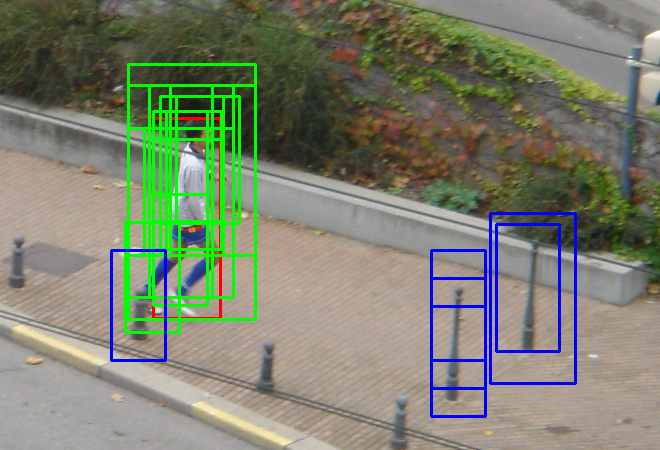
\includegraphics[width=0.9\textwidth]{ch4_dets.png}
\caption{Przykłady wyników klasyfikacji okien.}
\label{fig:detections}
\end{figure}


\section{Sposób bezpośredniego porównania metod}
\label{sec:porownanie}

Porównania skuteczności metod detekcji obiektów można dokonać poprzez
sprawdzenie jej działania na bardzo zróżnicowanym zbiorze testowym. W
kontekście tej pracy jest to zbiór różnych zdjęć, na których obecni są
ludzie w różnych pozach, w różnych częściach kadru, a także na
bardzo zróżnicowanym tle. Zastosowanie detekcji przy użyciu każdej z
poszczególnych metod pozwala na znalezienie zależności pomiędzy
odsetkiem fałszywych pozytywnych detekcji a skutecznością detekcji.
Sprawdzenie metody pod takim kątem pozwala na znalezienie konsensusu
pomiędzy stopniem fałszywych pozytywnych detekcji jakie można zaakceptować w konkretnym zastosowaniu, a celnością detekcji, jaką jesteśmy w stanie osiągnąć przy poszukiwaniu na obrazie konkretnej klasy obiektów. W rzeczywistych przypadkach bowiem,
z reguły nie ma się do czynienia ze wspomnianym przypadkiem detekcji na bardzo
zróżnicowanym zbiorze, lecz w stosunkowo niezmiennym środowisku, które
znane jest z góry. Wyznaczenie zależności pomiędzy częstością
występowania fałszywych pozytywnych detekcji w przypadku konkretnego
obrazu, a skutecznością metody pozwala zatem odpowiedź na pytanie - do
jakiego poziomu należałoby wytrenować klasyfikator, aby można było
uzyskać zadowalający oczekiwany stopień detekcji danej klasy obiektów.
Bardzo pomocnym narzędziem w tego typu analizie jest wyznaczenie
rozkładu błędu detekcji (DET - Detection error tradeoff), zaproponowanego w \cite{Martin97thedet}. Wykres, który służy do porównania między sobą klasyfikatorów binarnych, przedstawia zależność między odsetkiem fałszywych pozytywnych detekcji (reprezentowanej na osi odciętych wykresu), a stopniem nietrafionych pozytywnych detekcji danej metody (reprezentowanej na osi rzędnych wykresu). W przypadku dokonywania detekcji w przesuwnym oknie, jako odsetek fałszywych pozytywnych detekcji przyjmuje się rząd stosunku fałszywie pozytywnie zaklasyfikowanych okien do wszystkich badanych negatywnych okien (FPPW - False Positives Per Window). Wyższość jednej metody nad drugą, na podstawie wykresu DET, stwierdza się wtedy, gdy dla tych samych wartości fałszywie pozytywnych wskazań, wykres dla metody przyjmuje mniejszą wartość nietrafionych detekcji (krzywa opisująca rozkład lepszej metody jest na wykresie "pod" wykresem metody uznawanej za gorszą).

Oprócz tego, metody można bezpośrednio porównać wtedy i tylko wtedy
jeżeli dokona się detekcji w przesuwnym oknie z takim samym
przesunięciem okna w pionie i w poziomie w kolejnych detekcjach.
Ponieważ pożądana jest bardzo dokładne przebadanie zależności pomiędzy liczbą
FP a skutecznością detekcji liczba okien, w jakich
dokonywana jest detekcja przy użyciu każdej z metod powinna być taka
sama i możliwie jak największa.


\section{Analiza złożoności metod}
\label{sec:zlozonosc}

Zaproponowane metody różnią się między sobą m.in. operacjami matematycznymi potrzebnymi do obliczenia danego deskryptora czy długością wektora wynikowego.
Dlatego też, poza przeprowadzoną analizą jakościową,
przeprowadzono analizę czasową badanych metod. Badając każdą z nich
zmierzono czas, jaki był potrzebny dla wszystkich ww. etapów przeprowadzonych badań. Aby zapewnić wiarygodną porównywalność uzyskanych wyników wszystkie badania przeprowadzono na identycznej konfiguracji sprzętowej, a proces zajmujący się obliczeniami opisanymi w tym rozdziale był jedynym aktywnie działającym w systemie, przez co nie był on wywłaszczany przez inne procesy w kontekście czasu zajętości procesora.\\
Konfiguracja testowa była następująca:

\begin{itemize}
\item CPU: Intel(R) Xeon(R) CPU E5645 (4 x 2.40 GHz)
\item RAM: 14 GB
\item System operacyjny: Amazon Linux AMI 2012.09
\end{itemize}

W tym miejscu należy dodać, że sposób implementacji metod nie zapewniał zrównoleglenia ich obliczeń na wielu rdzeniach procesora. Toteż w trakcie uruchomienia testu, przy powyższej konfiguracji, w jednym czasie, aktywnie był wykorzystywany tylko i wyłącznie jeden rdzeń procesora.

\section{Podsumowanie}
\label{sec:podsmetodologia}
W celu podsumowania obranej metodologii przeprowadzonych badań, w tabeli \ref{tab:metodologia} zestawiono procedurę "krok po kroku" przyjętą w
metodologii analizy wybranych deskryptorów używanych w algorytmach
detekcji obiektów. Oprócz nazwanych etapów prowadzących do uzyskania
oceny danej metody uwzględniono informacje wejściowe potrzebne do
przeprowadzenia każdego z kolejnych kroków, jak i~informacje dostępne
na wyjściu, będące efektem przeprowadzenia danego etapu.

\begin{center}
    \begin{longtable}{ | l | p{4cm} | p{5cm} | p{5cm} |}
    \caption{Podsumowanie metodologii przyjętej w trakcie badania wybranych metod}
    \label{tab:metodologia}\\
    \hline
    Lp. & Nazwa kroku & Wejście & Wyjście \\ \hline
    1. & Generacja negatywnego zbioru testowego & Zbiór
negatywnych 1221 zdjęć (niezawierających sylwetek ludzkich) & Negatywne kadry treningowe 64x128 pikseli - kadr o największej ilości krawędzi
dla danego zdjęcia oraz 5 losowych kadrów \\ \hline

	2. & Ekstrakcja cech z pozytywnego zbioru treningowego &
	Pozytywny zbiór
kadrów treningowych o rozmiarze 64x128 pikseli 2419 &
	 Macierz
zawierająca 2419 wierszy, w każdym zawierająca wektor deskryptora cech \\ \hline

3. & Ekstrakcja cech z negatywnego zbioru treningowego &
   Negatywny zbiór
kadrów treningowych (wyjście z 1) o rozmiarze 64x128 pikseli &
Macierz
zawierająca 1221 wierszy, w każdym zawierająca wektor deskryptora cech \\ \hline

4. & Pierwszy trening klasyfikatora SVM &
Macierz cech pozytywnych (wyjście z 2) jako dane klasy 1, macierz cech
negatywnych (wyjście z 3) jako dane klasy 0 & Struktura SVM \\ \hline

5. & Walidacja krzyżowa pierwszego klasyfikatora & Struktura
wytrenowanego klasyfikatora SVM (wyjście z 4), zbiór pozytywnych (629) i
negatywnych (909)  kadrów testowych o rozmiarze 64x128 &
Skuteczność działania metody na pozytywnym i negatywnym zbiorze
testowym \\ \hline

6. & Znalezienie fałszywych pozytywnych wskazań dla metody & Zbiór
negatywnych (456) zdjęć & Negatywne kadry treningowe 64x128,
które pierwszy klasyfikator zaklasyfikował jako próbkę pozytywną\\ \hline

7. & Ekstrakcja cech ze zbioru fałszywych pozytywnych wskazań & Kadry
fałszywych pozytywnych wskazań dla metody & Macierz zawierająca n
wierszy, w każdym zawierająca wektor deskryptora cech\\ \hline

8. & Połączenie deskryptorów negatywnych cech & Macierz deskryptora
negatywnego zbioru treningowego (wyjście z 3, zawierająca 1221 wierszy),
macierz deskryptora fałszywych pozytywnych wskazań (wyjście z 7,
zawierająca m wierszy) & Wspólna macierz zawierająca 1221+m wierszy, w
każdym zawierająca wektor deskryptora cech \\ \hline

9. & Trening klasyfikatora SVM &
Macierz cech pozytywnych (wyjście z 2) jako dane klasy 1,  macierz
cech negatywnych (wyjście z 8) jako dane treningowe klasy 0 &
Dotrenowana struktura SVM\\ \hline

10. & Walidacja krzyżowa dotrenowanego klasyfikatora & Struktura
dotrenowanego klasyfikatora SVM,  zbiór pozytywnych i negatywnych
(629 + 909) kadrów testowych o rozmiarze 64x128 & Skuteczność
działania metody na pozytywnym i negatywnym zbiorze testowym po
dotrenowaniu \\ \hline

11. & Detekcja sylwetek ludzkich na obrazach testowych & Zestaw (629) obrazów testowych z sylwetkami ludzkimi wraz z opisem ich
umiejscowienia & Rozkład DET (liczba fałszywych pozytywnych detekcji do
stopnia celności) dla metody, wyniki detekcji dla poszczególnych
obrazów testowych\\ \hline
    
    \hline
    \end{longtable}
\end{center}